\chapter{Design}
\label{Chapter:Design}

This chapter discusses the design considerations during the design stage of the system. This stage of the development is very important since it lays down the foundation for the whole system.
Thus a considerable amount of time has been spent to carefully plan how the system should be designed. \citet[12]{bell2005} states that about 5\% of the total time that takes for the development of a software should be spent for the design state alone. For comparison, the coding process takes about 7\%; Testing takes 8\%. 

The design process has gone through many iterations to ensure the best possible quality of the product. The research presented in chapter \ref{Chapter:Literature-Review} has affected immensely the design, especially section \ref{section:commercial-har-systems}. The design can be split into four main sections, namely Mobile Platform and IDE; Database Design; Architectural design and User Interface (UI).

    

    \section{Mobile Platform and IDE}
    The first point that was considered in the design process was the \textbf{mobile platform} on which the proposed application will be implemented and distributed. After research on the current market, Google's \textit{Android} was found to dominate in Europe \citep{williams2016}. Android-based smartphones hold 75.6\% of market share dominating other mobile platforms such as Apple's \textit{iOS} and Microsoft's \textit{Windows Phone}. Thus, Android OS was chosen to form the basis of the proposed mobile application since it allows the application to be downloaded and used by as many people as possible.
        
    After choosing the mobile platform, the development environment or the \textbf{Integrated Development Environment} (\gls{ide}) which is a software that will be used to develop the application. That was an easy decision since \textit{Android Studio} is known to be the official \gls{ide} for Android development \citep{androidstudio2017}. It provides all the necessary developer tools such as \textit{Android Emulator} which is a basically a virtual phone that allows a developer to test an application on different versions of the platform. In addition, it supports direct integration of version control systems such as \textit{Git}.
    
    \section{HAR}
    The Human Activity Recognition process involves standard stages such as \textit{Data Preprocessing}, \textit{Feature Extraction} and \textit{Feature Selection} (see section \ref{section:feature-selection&extraction}). The block diagram of the \gls{har} process can be seen in figure \ref{fig:har_process}. Weka\footnote{\url{http://www.cs.waikato.ac.nz/ml/weka/}} Data Mining Software has been chosen for the implementation of the \gls{har} component of the proposed system. Since there is no official support of the Weka API on the Android platform, a stripped-down version\footnote{\url{https://github.com/rjmarsan/Weka-for-Android}} of the original Weka Java API has been chosen. This library was tested prior to the design stage to ensure it functions well on an android device. 
    
    \begin{figure}[H]
        \centering
        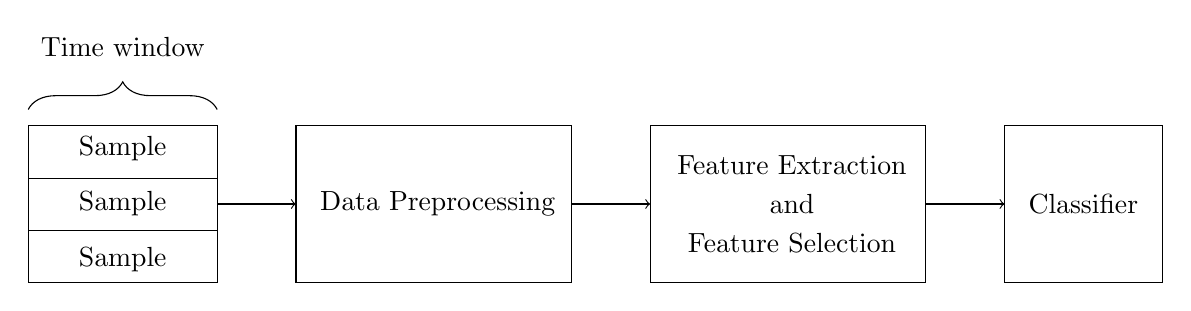
\begin{tikzpicture}
            \node at (1.2,3) {Time window};
            \draw (0,0) rectangle (2.4,2);
            \draw [decorate,decoration={brace,amplitude=10pt}] (0.0,2.2) -- (2.4,2.2); 
            \draw (0,0.66) -- (2.4,0.66);
            \draw (0,1.32) -- (2.4,1.32);
            \node at (1.2,1) {Sample};
            \node at (1.2,0.3) {Sample};
            \node at (1.2,1.7) {Sample};
            \draw [->] (2.4,1) -- (3.4,1);
            \draw (3.4,0) rectangle (6.9,2);
            \node at (5.2,1) {Data Preprocessing};
            \draw [->] (6.9,1) -- (7.9,1);
            \draw (7.9,0) rectangle (11.4,2);
            \node at (9.7,1.5) {Feature Extraction};
            \node at (9.7,1) {and};
            \node at (9.7,0.5) {Feature Selection};
            \draw [->] (11.4,1) -- (12.4,1);
            \draw (12.4,0) rectangle (14.4,2);
            \node at (13.4,1) {Classifier};
        \end{tikzpicture}
        \caption{Human Activity Recognition process}
        \label{fig:har_process}
    \end{figure}
    
    \subsection{Dataset}
    As it was mentioned in section \ref{section:proposed-application}, \textit{"Active Minutes"} is using a \textit{Supervised} learning method. This learning method require a labeled \textit{"training data"} or \textit{"data set"} order to build a classifier (or model). After a classifier is build it can be used to classify \textit{"unseen"} or \textit{"unlabelled"} data.
    
    
    \subsection{Data Processing}
    The data processing stage of \gls{har} normally involves segmenting the data into time windows. Considering the fact that the system will be running on a mobile device with limited resources, the window length has to be picked carefully. For example, choosing a 20-second window length (see figure \ref{fig:har_process}) will cause the CPU to do more work due to the amount of \textit{samples} in the time window. Consequently, that would lead to a higher battery consumption \citep[2]{torreshuitzil2015a}. As it was found in the literature review (see section \ref{section:learning_alg_accuracy_power_consm}), 3-second time window produces good results in terms of power consumption. Based on those findings, the proposed application will adopt this window length as well.
    
    During this stage, different filters could be applied to the raw data to remove unwanted information. For example, according to \citet[]{googlemotionsensors}, the raw data from an accelerometer sensor contains the earth's gravity force as well. This will cause the device to read magnitude of g = 9.81 m/s2 when it is not accelerating (i.e. laying down on a table). In order to obtain just the linear acceleration without natural forces (i.e. earth's gravitation), a low-pass filter is applied.
    
    In order to reduce the effect of device location (e.g. where the device is ) the magnitude of the accelerometer's x,y and z axis is also calculated during this stage and used as a 4th axis \textit{"m"} (see equation \ref{eq:acceleration_magnitude} bellow). This technique has been used in previous works as well \citep[153]{torreshuitzil2015b}.
    
    \begin{equation}
        \label{eq:acceleration_magnitude}
        m = \sqrt{x^2 + y^2 + z^2}
    \end{equation}
    
    \subsection{Feature Extraction and Feature Selection}
    \textbf{Feature extraction} is an important process in a \gls{har} system. It allows extracting key characteristics from a raw data and used to represent important patterns with reduced dimensionality \citep[154]{torreshuitzil2015b}. During the initial research (see section \ref{section:feature-selection&extraction}) it was found that extracting the first \gls{fft} algorithm coefficients produce higher accuracy compared to the rest of the features (e.g. Time domain features such as Mean or Standard Deviation). To ease the development process, a third-party library called \textit{JTransforms} \footnote{\url{https://github.com/wendykierp/JTransforms}} has been utilised to convert the Time-Domain raw accelerometer data (data collected over a time period) into a Frequency-Domain data by applying the above-mentioned algorithm. The total number of features that are extracted from the raw accelerometer sensor is 20. That includes the first 5 \gls{fft} coefficients of the x,y and z axis as well as their magnitude. 
    
    \textbf{Feature selection} algorithms can be applied after the Feature Extraction process to reduce the number of features, and thus simplifying the classifier (see section \ref{section:feature-selection&extraction}). The main goal of the feature selection algorithm is to select a subset from the original data features that can accurately carry the original meaning of the data \citep[22]{wu2008}. For example, if the original number of features is 20 after applying a feature selection algorithm that number could be reduced to 13 which would lead to a faster CPU processing. A Correlation based Feature Selection (CFS) algorithm has been chosen for the implementation of the feature selection process since it showed good results in previous works \citep[220-224]{dinhle2015}. The \gls{cfs} algorithm selects a subset of features based on two factors. First the algorithm calculates the correlation between the feature-class and feature-feature. The feature-class correlation shows how much a feature is related to a certain class (i.e. such as \textit{"walking"} or \textit{"static"}). On the other hand, the feature-feature correlation shows how individual features relate to each other.
    
    \subsection{Classifier}
    After the Data Processing and Feature Extraction and Feature Selection stages a classifier is built. The initial research suggested the use of the k-Nearest Neighbors (kNN) algorithm to build the classifier due to the fact that it does not require much CPU work and thus it is battery friendly (see \ref{section:learning_alg_accuracy_power_consm}). Based on those findings, the proposed mobile system will employ the same learning algorithm. 
    
        
    \section{Architectural design}
    \label{section:architectural-design}
    This section discusses the software software architecture of the mobile application. The architectural design is the first stage in the design process of a system. It creates a critical link between the requirements discussed in Chapter \ref{Chapter:Specification} and the research knowledge gained in Chapter \ref{Chapter:Literature-Review}. The end-goal of the architectural design is to discover the major structural components of the system and how they communicate to each other \citep[148]{sommerville2010}. The architectural model of the system can be seen in figure \ref{fig:architectural_design_component_diagram}.
    
    \begin{figure}[H]
        \centering
        \includegraphics[width=15cm]{active-minutes-service-component-diagram}
        \caption{ \textit{"Active Minutes"} Architectural model (simplified)}
        \label{fig:architectural_design_component_diagram}
    \end{figure}
    
    Model-View-Presenter or \textbf{MVP} software architectural pattern was chosen to form the base of the proposed mobile system since it provides clean separation of concepts \citep[532]{zhang2010}. For example the \textit{View} represents the \gls{ui} of the application. It contains logic for receiving user interaction and notifying the \textit{Presenter}. The \textit{Model} is the data layer. It is responsible for providing and formatting (i.e. applying the business logic to) the data and returning it to the Presenter. The \textit{Presenter} acts as a mediator, it requests data from the \textit{Model} and returns it to update the \textit{View}. Figure \ref{fig:model_view_presenter_design_pattern} shows the interaction flow of the pattern. When the user interacts with the \gls{ui} of mobile application, the View receives the interaction (i.e. button click) and passes that information to the Presenter via Interface (\textit{IView}). The Presenter then invokes the appropriate method of the Model. Next, the Model returns the requested data to the View (via the Presenter). 
        
    The main \textbf{advantages} of using the \gls{mvp} pattern is that it increases the \textbf{testability} of the software via the concept of logic separation. For example, the View is only allowed to have framework specific code (i.e. Android UI components such as Button, ListView); Presenter and Model are comprised of Plain Old Java Objects or \textbf{POJO}. These POJO classes can be thoroughly tested outside the mobile application. In addition, the \gls{mvp} pattern introduces a certain level of abstraction in the software architecture via the use of Java Interfaces such as \textit{ILoginView} (see figure \ref{fig:architectural_design_component_diagram}). That allows different parts of the software to be developed separately and then integrated into the application. The components of the system will be discussed in the following sections.
    
    \begin{figure}[ht]
        \centering
        \includegraphics[width=15cm]{model-view-presenter-design-pattern}
        \caption{Model-View-Presenter design pattern \citep[28]{syromiatnikov2014}}
        \label{fig:model_view_presenter_design_pattern}
    \end{figure}
        
        \subsection{Models}
        As it can be seen from figure \ref{fig:architectural_design_component_diagram} the \textit{Model} layer of the system architecture is comprised of \textit{DataManager}, \textit{ActiveMinutesService}, \textit{ClassifierPersonalisationService} and \textit{DataCollectionService}. These components will be discussed next.
        
            \subsubsection{DataManager}
            \label{section:data-manager}
            The \textbf{\textit{DataManager}}, as the name implies, is responsible for providing means of accessing the underling database object. For example, retrieving a list of activities for the logged-in user. Almost all of the diagram components have access to DataManager. Thus they can perform operations such as saving a new user or loading user's physical activity goal. This class essentially is a wrapper of a \textbf{Realm} database object. After initial research, \citet{realm2014} was chosen to form the database of the mobile application. It is a third-party Android library found to be x100 faster compared to the Android native SQLite Object-Oriented Data Management System (OMS).
            
            \subsubsection{ActiveMinutesService}
            \label{section:active-minutes-service}
            Since \textit{"Active Minutes"} has to collect contextual information throughout the user's day continuously, \textbf{\textit{ActiveMinutesService}} is implemented as an Android \textit{Service} class. According to \citet{googleservices2017}, a Service is an application component that continuously runs in the background even if the user closes or switches to another application. The responsibilities of this service include \gls{har}, storing the recognised activities in the database and performing additional checks such as whether or not to send reminder notification to the user for sitting for too long.
            
            Another important responsibility of the this service is to collect personal data. This data is used later on for classifier personalisation (e.g. adapting the general classifier so it better recognises user activities).
            
            \subsubsection{ClassifierPersonalisationService}
            The sole purpose of this service is to personalise the general classifier that is included in the application initially. It will be started by the above mentioned \textit{ActiveMinutesService} service when enough labeled data is collected. For example, the service is executed when there are x100 instances of \textit{walking},\textit{running}, \textit{cycling} and \textit{static} activity training data. Since it will run once in the lifetime of the application on the device, this service is implemented as a special kind of Service called \textit{IntentService}. It allows for execution of heavy tasks (such as training a classifier) in a worker (i.e. background) thread so the application's main thread (or \gls{ui} thread) is not affected.
            
            \subsubsection{DataCollectionService}
            \label{section:data_collection_service}
            In order to train a \gls{har} classifier, a training dataset is required. This service is responsible for the data collection process. That includes reading, prepossessing and windowing the raw accelerometer data as well as abstracting the data via the means of feature extraction (see section \ref{section:feature-selection&extraction}). Each feature vector stores 20 values (the first 5 \gls{fft} coefficients of every sensor axis, namely x,y and z and their magnitude) as a record in the \textit{Training\_data} table (see figure \ref{fig:data_modeling_er_diagram}).
            
        \subsection{Views}
        The View layer of the \gls{mvp} pattern is comprised of Interface classes that are implemented by Android components such as \textit{"Activity"} or \textit{"Fragment"}. This approach provides a layer of abstraction and logic separation which is one of the benefits of using the \gls{mvp} design pattern. From an Android standpoint, an \textit{Activity} is a class that creates a window (e.g. single screen) and its layout (a specific arrangement of \gls{ui} components such as \textit{"Buttons"}) can be set via using the method \textit{"setContentView(View)"} \citep{googleactivity2017}. According to \citet{googlefragments2017}, \textit{"Fragment"} is a \textit{"sub-activity"} like class with its own layout. They can be swapped with one another easily thus they are highly reusable. Fragments typically require a host Activity in order to be presented to the user. For example, the \textit{"LoginFragment"} and \textit{"SignupFragment"} are hosted in an Activity called \textit{"AuthenticationActivity"}. As it can be seen from figure \ref{fig:architectural_design_component_diagram} all of the \textit{View}s in the \gls{mvp} pattern communicate with a dedicated Presenter class in the \textit{Presenter} layer via an interface. The following sections will describe what are the responsibilities of each one of those components.
            
            \subsubsection{AuthenticationActivity}
            As the name of the component suggests, this is a Android \textit{Activity} class that handles the login and sign up functionality of the application. This activity is responsible of presenting the two fragments it hosts, namely \textit{"LoginFragment"} and \textit{"SignupFragment"}. The LoginFragment is responsible of checking the login user credentials and eventually transferring the user to the main screen of the mobile application. As for the SignupFragment, it handles the process of creating a new user.
            
            \subsubsection{ActiveMinutesActivity}
            The main purpose of this activity is to display the contents of the \textbf{"TodayFragment"} (e.g. Today screen) and \textit{"HistoryFragment"} (e.g. History screen). The TodayFragment shows current information to the user such as how much time a user has been active today ( as well as details for individual activities, see section \ref{section:user_interface_design}).
            
            The \textbf{HistoryFragment} is responsible for showing the log of activities both daily and weekly. This way the user can refer to a previous day in time if needed.
            
            \subsubsection{DataCollectionActivity}
            This Android \textit{Activity} class is responsible for providing an interface for controlling the \textit{DataCollectionSertice} mentioned in section \ref{section:data_collection_service}. It's \gls{ui} provide buttons for starting and stopping the service as well as exporting the acquired data into a labeled dataset file format - \textit{ARFF}. Later on this file will be used to build a classifier using the machine learning library WEKA.
            
            \subsubsection{SettingsFragment}
            As the name implies, this Fragment class is responsible for providing the user with the ability to change certain parameters of the application. For example, the user can change the default \gls{pa} goal as well as the \textit{"Sleeping Hours"} time window.
            
            
        \subsection{Presenters}
        The \textit{Presenter} layer of application's architecture is comprised of a set of Presenter classes (see figure  \ref{fig:architectural_design_component_diagram}) associated with the different screens of the application.
    
    \section{Database Design}
    \label{section:database-design}
    This section discuses the design of the database system that will be used to store data of \textit{"Active Minutes"} mobile application. The design of the database can be seen in figure \ref{fig:data_modeling_er_diagram}. It includes the following entities \textbf{User}, \textbf{Activity} and \textbf{Training\_data}. The following sections will explain the responsibilities of each entity (i.e.\ database tables).
        
        \begin{figure}[ht]
            \centering
            \includegraphics[width=12cm]{data-modeling-er-diagram}
            \caption{Database ER Diagram}
            \label{fig:data_modeling_er_diagram}
        \end{figure}
        
        \subsubsection{Entities}
        
        \begin{itemize}
            \item User(user\_id, password, username, pa\_goal,max\_cont\_inac\_goal, is\_classifier\_personalised, profile\_picture)
            \item Training\_data(user\_id, acc\_x\_fft\_1, acc\_x\_fft\_2, acc\_x\_fft\_3, acc\_x\_fft\_4...)
            \item Activity(activity\_id, user\_id, type, date, duration)
        \end{itemize}
        
        \subsubsection{Relationships}
        \begin{itemize}
        \item Does --- User does Activity [1:m][m:o]
        \item Produces --- User produces Training\_data [1:m][m:o]
        \end{itemize}
        
        \subsection{User}
        The user table is responsible for storing the personal information of every registered user. For example, \textbf{\textit{user\_id}} allows every user to be uniquely identified in order to access other details such as \textbf{\textit{username}} and \textbf{\textit{password}}. These fields are used to authenticate different users of the application upon login.
        
        The user table stores additional information such as the \gls{pa} goal (\textbf{\textit{pa\_goal}}) and the maximum continuous inactivity goal (\textbf{\textit{max\_cont\_inac\_goal}}). The table also stores a Boolean field called \textbf{\textit{isClassifierPersonalised}}. This field is set to \textit{False} by default and only changed when the general classifier, bundled with the application, is personalised with user's data. Since every user sets their \textit{Sleeping Hours} by design (i.e. a time window during which the user would not be monitored) fields called \textit{startSleepingHours} and \textit{stopSleepingHours} are needed to store the start and stop sleeping hours set by the user. Last but not least, fields called \textbf{\textit{profile\_picture}} and \textbf{\textit{isFirstTime}} are responsible for storing the user's profile image and if the user uses the application for the first time, respectively.
        
        \subsection{Activity}
        As it can be seen from figure \ref{fig:data_modeling_er_diagram}, the Activity table is responsible for storing information for the different activities. Every table record is created once every day. Once created, its fields are amended accordingly throughout the day depending on the amount of \gls{pa} and \gls{st}. 
        
        Every activity record in the table has a unique identifier \textbf{\textit{activity\_id}} that uniquely identifies it. Also, the table stores the user's id in a field called \textbf{\textit{user\_id}}. That allows for associating a given activity record with a specific user.
        
        The table is also storing fields that store user's activity levels. For example, \textbf{\textit{active\_time}} field stores the amount of \gls{pa} the user is accumulated for a specific day. Other table fields are responsible to storing statistical information regarding sedentary information such as \textit{longest\_inactivity\_interval}, \textit{currentInactivityInterval}, \textit{averageInactivityInterval} and \textit{totalInactivityTime}. In addition, a field called \textit{timesCurrentInactivityReset} is used to store how many times the current inactivity is being reset (needed to calculate the average inactivity interval).
        
        
        \textbf{\textit{Activity}} table also stores user's \gls{pa} goal represented by \textit{user\_pa\_goal} as well as \gls{st} goal represented by \textit{user\_max\_cont\_inac\_goal}.
        
        \subsection{Training\_data}
        The last database table to discus is the Training\_data. The fields from the table \textbf{\textit{acc\_x\_fft\_1}},\newline\textbf{\textit{acc\_x\_fft\_2}},\textbf{\textit{acc\_x\_fft\_3}}... are responsible for storing the extracted features from the raw accelerometer data as discussed in section \ref{section:proposed-application}. The table field \textbf{\textit{user\_id}} is used to associate a user with a particular record in the table. \textit{ClassValue} field stores label of the training data record (i.e. walking).
        
        One point to note, this table will be used for two purposes at different times of the development of the project. First, it will be used to store all of the project participants training data. This data will be used to build an initial, general classifier. When a classifier is already build, this table will be used to store the labeled data that will be used to build a personalised classifier for a particular user.
    
    
        
    \section{User Interface Design}
    \label{section:user_interface_design}
    The process of designing a user interface is highly dependent on the system's specifications discussed in chapter \ref{Chapter:Specification}. For example, the application requires user authentication thus a design for the login and sign up screens have been considered. A \gls{ui} design process proposed by \citet[60]{bell2005} has been applied in this work (see figure \ref{figure:ui-design-process}). According to Bell, the \gls{ui} design process is usually informed by certain design principles and guidelines to make sure that the application is user-friendly. Next, prototyping tools are used to create a system prototype which is evaluated by the user for quality. That is followed by implementing the user's feedback into the prototype. This process is repeated until the user is happy with the prototype of the system. The following sections will discuss how the mobile's application \gls{ui} was achieved as well as what design principles and guidelines have been considered.
    
    \begin{figure}[ht]
    \centering
        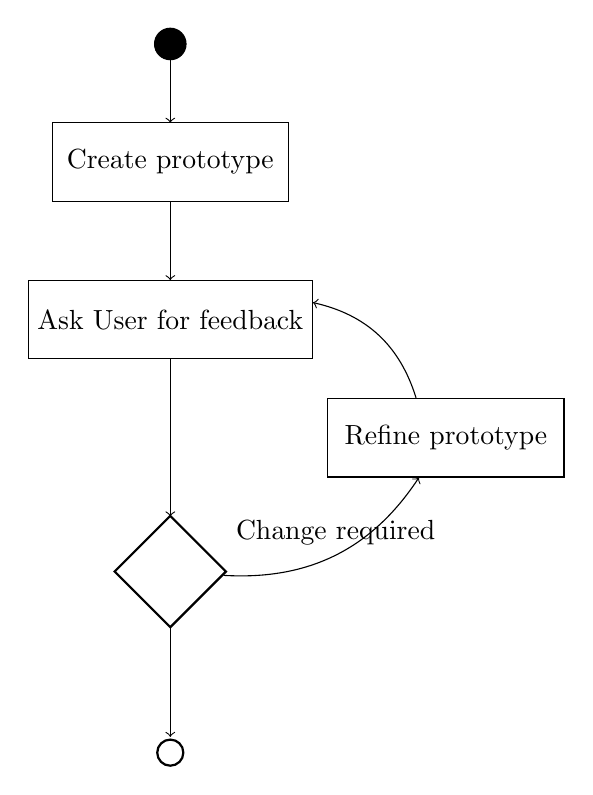
\begin{tikzpicture}
            \draw[fill=black] (0,0) circle (0.2);
            \draw [->] (0,0) -- (0,-1);
            \draw (-1.5,-1) rectangle (1.5,-2);
            \node at (0,-1.5) {Create prototype};
            
            \draw [->] (0,-2) -- (0,-3);
            \node (check) [draw, shape=rectangle, minimum width=2.5cm, minimum height=1cm, anchor=center] at (0,-3.5) {Ask User for feedback};
            
            \draw [->] (0,-4) -- (0,-6);
            \node (usercheck) [draw, thick, shape=rectangle, minimum width=1cm, minimum height=1cm, anchor=center,rotate=45] at (0,-6.7) {};
            
            \node (ref) [draw, shape=rectangle, minimum width=3cm, minimum height=1cm, anchor=center] at (3.5,-5) {Refine prototype};
            
            \draw [->] (0,-7.4) -- (0,-8.8);
            \node (end) [draw, thick, shape = circle, minimum width = 0.3cm] at (0,-9) {};
            
            \draw[->, to path={-| (\tikztotarget)}]
            (ref) edge[bend right] node [left] {} (check) 
            (usercheck) edge[bend right] node [pos=.5,above] {Change required} (ref);
            
        \end{tikzpicture}
    \caption{Iterative process of UI prototyping}
    \label{figure:ui-design-process}
    \end{figure}
    
        \subsection{System Prototyping}
        In order to create the system prototype, a set of wireframes were created (see appendix \ref{chapter:screen-wireframes}). Next, the wireframes were further developed into a \gls{ui} design. Both the wireframe and user interface designs were created using a software design tool called \textit{Sketch}\footnote{\url{https://www.sketchapp.com/}}. The design of every mobile screen can be seen in appendix \ref{chapter:screen-design}. 
        
        After the design of the mobile screens was completed. A software called \textit{Flinto}\footnote{\url{https://www.flinto.com/}} was used to create a system prototype. One of the reasons of choosing \textit{Sketch} as a design tool is because it allows for easy export of Sketch pages to \textit{Flinto} documents thanks to a dedicated plugin.
        
        In order to create the prototype, special objects called \textit{Links} had to be drawn over the mobile screen designs (i.e. buttons). Every link needs a target to be specified. For example, in figure \ref{fig:flinto_prototype}) there is a link object drawn over the \textit{"Weekly"} button and its target is set to be the whole \textit{"History Screen Weekly"} screen. So when the user inspects the design prototype and presses the \textit{Weekly} button they will be taken to the other screen. This process of creating links and targets was used in order to create a fully functioning system prototype that the user can interact with and gain a clearer idea of how the system could be implemented.
        
        \begin{figure}[ht]
            \centering
            \includegraphics[width=12cm]{flinto-screen-links}
            \caption{Flinto prototype creation process}
            \label{fig:flinto_prototype}
        \end{figure}
        
        
        \subsection{Design Principles and Guidelines}
        
        \subsubsection{Design Principles}
        Design principles are well-accepted principles that can inform how a user interface is being designed. Platform specific principles have informed the system design. For example, the first design principle suggested by \citet{google2017b} \textbf{"Delight me in surprising ways"} have been implemented in the authentication screens as the ability of the user to change screens via a swipe gesture. This action is reflected by the \textit{page indicator} at the bottom of the screens (see figure \ref{fig:authentication-screens}). According to Google, subtle effects such as these contribute to a feeling of effortless. 
        
        \textbf{"Only show what I need when I need it"} is another principle suggested by \citet{google2017b}. It focuses on the fact that people get confused when presented with a lot of information at once. \textit{"Active Minutes"} incorporates this principle by providing a \textit{"Navigational Drawer"} that provides additional options for the user such as \textit{"Settings"} and \textit{"Log Out"} buttons and when not needed it could be hidden (see figure \ref{fig:nav-drawer-opened}). 
        
        \textbf{"I should always know where I am"} is a principle that allows the user to gain confidence that they know how how to use the system. For example, when switching between the \textit{Login} and \textit{Signup} screens the text of the button is changed to \textit{"LOG IN"} and \textit{"SIGN UP"} accordingly so the user can infer where they are at the moment (see figure \ref{fig:authentication-screens}).
        
        As per system specifications, the system will notify the user when a goal is met (see section \ref{section:feedback-component}). The next principle \textbf{"Only interrupt me if it's important"} implies that the user should not be interrupted unless it is important. For example, the system sends a notification when a prolonged sedentary time is recognised. In this case, the user must be notified so they can take action.
        
        \subsubsection{Design Guidelines}
        \citet[57-59]{bell2005} states that Design Guidelines need to be considered in the context of the platform the software is being designed for. Since \textit{"Active Minutes"} is developed as an Android application, it needs to comply with the platform specific design guidelines. That is why the system design has been informed by the official Android design guidelines \citep{googleamaterialdesign}. Google's new design language called \textit{"Material Design"} have been applied to the design of the application. It provides various guidelines such as the ideal layout metrics to be used when designing a \textit{Navigation Drawer}. 